\section{Simulation}
\label{sec:sim}
%%%%%%%%%%%%%%%%%%%%%%%%%%%%%%%%%%%%%%%%%%%%%%%%%%%%%%%%%%%%%%%%%%%%%%%%%%%%%%%%%%%%%%%%%%%%%%%%%%%%%%%%%%%%%%%%%%%%%%%%
In this section we present the Monte Carlo simulation study that was performed to optimize the 
geometry and performance of the LXe scintillation detection system. We perform a GEANT4 based 
simulation to obtain the reasonable dimensions of the spherical LXe holder and the placement of 
the PMT detectors around it, which is described in section \ref{subsec:DetGeometry}. In 
section \ref{subsec:StatAnalysis}, we discuss the statistical test performed to find the 
detector's sensitivity in measuring various patterns of the scintillation emission from 
the LXe target.

%%%%%%%%%%%%%%%%%%%%%%%%%%%%%%%%%%%%%%%%%%%%%%%%%%%%%%%%%%%%%%%%%%%%%%%%%%%%%%%%%%%%%%%%%%%%%%%%%%%%%%%%%%%
\subsection{The Detector Geometry}
\label{subsec:DetGeometry}
 We perform a study to optimize the dimensions of the setup using a GEANT4 based framework
 that includes realistic description of the  target, the enclosing HPFS sphere and the PMTs 
 around. The simulations takes into account the physics processes of the propagation of the photons 
 from the LXe  target through the the sphere and the vacuum and their interaction at the PMTs. 
 The parameters under test for this study are the size of the sphere, the PMT size and their 
 placement around the sphere. The refractive index and internal transmittance of both 
 of LXe and of HPFS are known with good precision. 
 
 For the simulation, we fix all parameters except the outer radius ($R_{2}$) of the sphere. The fixed 
 parameter values are chosen by quantitative physical considerations and educated guesses.
The radius of the LXe target $R_{1}$ will determine the event rate for a particular 
source, and we choose it to  be 1 cm. The conventional PMTs designed by Hamamatsu to 
detect scintillation from LXe are 1'' and 3'' square PMTs, and we choose the 1' ones in order 
to get better spatial resolution. an array of 20 PMTs around the sphere, placed at a distance of 
39 mm from the centre of the targetare considered. The active area of each PMT is 22 mm $\times$ 22 mm.

\begin{table}[h]
  \centering
  \caption{The optical parameters used in simulation}
  \label{tab:OptPar}
  \begin{tabular}{|c|c|}
  \hline
  Parameter & Value\\
  \hline
  LXe absorption length & 100 cm\\
  \hline
  LXe scattering length & 35 cm\\
  \hline
  HPFS absorption length & 100 cm\\
  \hline
  HPFS scattering length & $\infty$ \\
  \hline
  LXe refractive index & 1.61 \\
  \hline
  HPFS refractive index & 1.57 \\
  \hline
  \end{tabular}
\end{table}

In order to chose a reasonable dimension of the sphere, we first study the detection efficiency of 
scintillated photons in the simulated setup. Using an inotropic emmision of 50photons/event, we find 
the average ratio of the detected photons/event to the net emitted photons/event, for various choices 
of $R_{2}$. The trasmittance of HPFS is a crucial parameter and we vary it within a large range to 
check the impact of it. The photon detection ratio for different sets of $R_{2}$ and transmittance are 
shown in Fig.~\ref{fig:pdr}.  At very low R$_{2}$ the total internal reflections causes the number of photons emerging from 
the sphere to drop. As the R$_{2}$ increases the total internal reflections decreases resulting in an 
increase in the number of photons croosing the sphere. After certain increase in R$_{2}$, the transmittance 
of HPFS becomes the dominant factor and the photon detection ratio starts falling. This is an important factor 
to chose a suitable value of R$_{2}$.

\begin{figure}
   \centering
   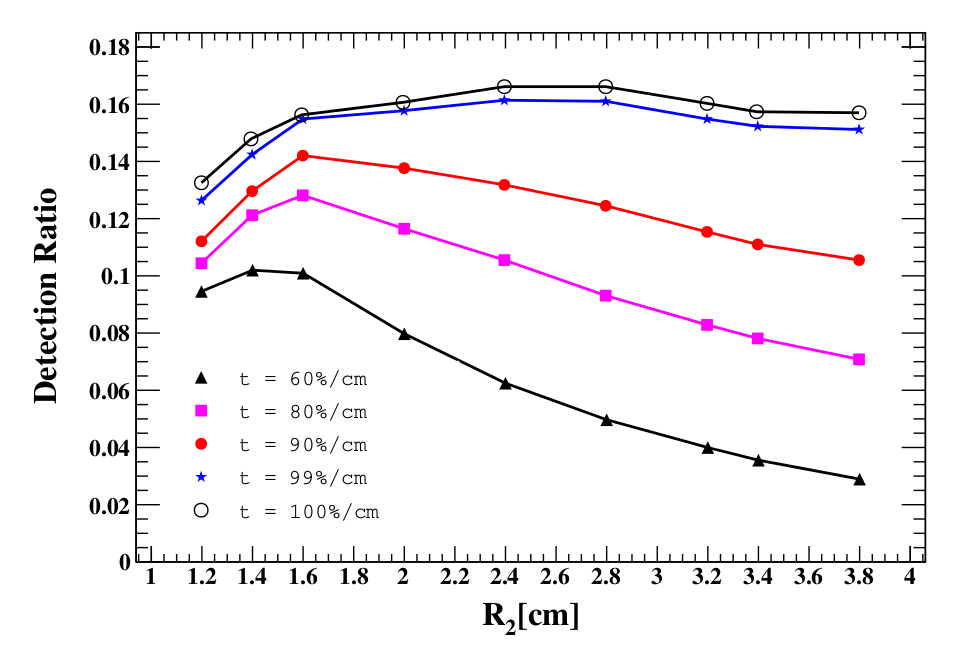
\includegraphics[width=0.5\textwidth]{pdr.png}
   \caption{The photon detection ratio as a function of R$_{2}$, for different transmittances of 
   the fused silica shell. We use 10$^4$ events with 50 photons/event for each choice of transmittance 
   and R$_{2}$. At very low R$_{2}$ the total internal reflections causes the number of photons emerging from 
   the sphere to drop. As the R$_{2}$ increases the total internal reflections decreases resulting in an 
   increase in the number of photons croosing the sphere. After certain increase in R$_{2}$, the transmittance 
   of HPFS becomes the dominant factor and the photon detection ratio starts falling.}
   %drops.
   \label{fig:pdr}
\end{figure}

%%%%%%%%%%%%%%%%%%%%%%%%%%%%%%%%%%%%%%%%%%%%%%%%%%%%%%%%%%%%%%%%%%%%%%%%%%%%%%%%%%%%%%%%%%%%%%%%%%%%%%%%%%%%%%%%%%%%%%%%%%%%
\subsection{The statistical test}
\label{subsec:StatAnalysis}
In this section, we present the study on the ability of the proposed detector to detect the emission pattern 
of the LXe scintillation with a high statistical significance. For each scintillation event, the PMTs 
will detect only a certain fraction of the total photons produced. We pick a few cases of emission 
patterns as shown in Table~\ref{tab:emissionpattern},

\begin{table}[h]
  \centering
  \caption{The emission patterns used in simulation}
  \label{tab:emissionpattern}
  \begin{tabular}{|c|c|c|c|}
  \hline
  Pattern no. & Beam specification & Beam Half widths & Signal fractions\\
  \hline
  LXe absorption length & 100 cm\\
  \hline
  LXe scattering length & 35 cm\\
  \hline
  HPFS absorption length & 100 cm\\
  \hline
  HPFS scattering length & $\infty$ \\
  \hline
  LXe refractive index & 1.61 \\
  \hline
  HPFS refractive index & 1.57 \\
  \hline
  \end{tabular}
\end{table}